\documentclass[11pt,a4paper]{article}
\usepackage[spanish,es-tabla]{babel}
\usepackage{subcaption} 
\usepackage[utf8]{inputenc} % Escribir con acentos, ~n...
\usepackage{eurosym} % s´ımbolo del euro
\newcommand{\horrule}[1]{\rule{\linewidth}{#1}} % Create horizontal rule command with 1 argument of height\usepackage{listings}             % Incluye el paquete listing
\usepackage[cache=false]{minted}
\usepackage{graphicx, float} %para incluir imágenes y colocarlas
\usepackage{epstopdf}
\usepackage{natbib}
\usepackage{hyperref}
\hypersetup{
	colorlinks,
	citecolor=black,
	filecolor=black,
	linkcolor=black,
	urlcolor=black
}
\usepackage{multirow}
\usepackage{array}
\usepackage{diagbox}
\usepackage{minted}


\title{
\normalfont \normalsize 
\textsc{{\bf Servidores Web de Altas Prestaciones (2019-2020)} \\ Grado en Ingeniería Informática \\ Universidad de Granada} \\ [25pt] % Your university, school and/or department name(s)
\horrule{0.5pt} \\[0.4cm] % Thin top horizontal rule
\huge 
Máquina virtual preparada para ponerla en hardware anfitrión \\ Nº 32 % The assignment title
\horrule{2pt} \\[0.5cm] % Thick bottom horizontal rule

\includegraphics{images/logo.png}	
}

\author{Antonio Jesús Heredia Castillo \\ José Manuel Pérez Lendínez \\ Miguel Ángel Hinojosa Castro \\ Se dedicaron 12 horas a la realización del trabajo} % Nombre y apellidos

\date{\normalsize\today} % Incluye la fecha actual

%----------------------------------------------------------------------------------------
% DOCUMENTO
%----------------------------------------------------------------------------------------

\begin{document}

\maketitle % Muestra el Título
\newpage %inserta un salto de página
\tableofcontents % para generar el índice de contenidos
\listoffigures
\newpage
\section{Introducción}
Docker es una plataforma de código abierto que ejecuta aplicaciones y hace que desarrollar, distribuir y desplegar sea mucho más sencillo. Esto es posible debido a que las aplicaciones se empaquetan con todas las dependencias de soporte en un marco estándar llamado contenedor. Estos contenedores funcionan de forma aislada entre sí y muy por encima del núcleo del sistema operativo.

En nuestro proyecto, vamos a dar unas pinceladas de algunas funciones de Docker, así como otras alternativas que existen en el mercado y que utilizan la virtualización de contenedores. Además, vamos a realizar tres ejemplos de diferente índole para ilustrar el desarrollo de aplicaciones en Docker y de algunos de sus competidores.

Antes de entrar en más detalle, vamos a realizar una pequeña introducción a las maquinas virtuales, ya que creemos fundamental entender bien su funcionamiento para ver la importancia que estas tienen.
\section{Antecedentes}
Una máquina virtual se implementa añadiendo una capa de software a una maquina real para soportar la arquitectura de la maquina virtual deseada. Este proceso se conoce como virtualización. Además, la virtualización hace posible tener varias maquinas virtuales en un mismo recurso hardware. Esto nos permite tener entornos aislados, favoreciendo así propiedades como la seguridad.\\\\
 Generalmente nos referimos a la plataforma sobre la que se ejecuta como ``host'' o anfitrión y al software que se ejecuta en la \textbf{VM} como ``guest'' o invitado (ver Figura \ref{fig:1.6}).
 \begin{figure}[H]
	\centering
	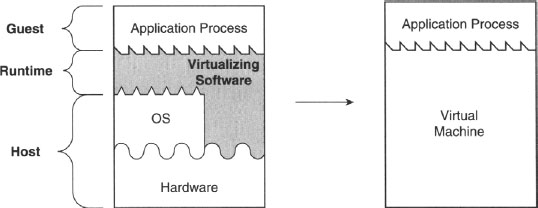
\includegraphics[scale=0.75]{images/fig16.jpg}
	\caption[Transformación de un SO a una VM]{Transformación de un SO a una VM.}
	\label{fig:1.6}
\end{figure}
 El software de virtualización a menudo se conoce como ``runtime'', este es creado para soportar al proceso invitado y corre sobre el sistema operativo. Esto sería  una perspectiva de proceso. Aquí encontramos varios subtipos:
 \begin{itemize}
     \item Multiprogramación.
     \item Emuladores y traductores dinámicos de binarios.
     \item Optimizadores binarios.
     \item Maquinas virtuales de lenguajes de alto nivel.
     
 \end{itemize}
Por otro lado, existen ``sistemas de máquinas virtuales'', que nos proveen un entorno completo. Que nos brindan un sistema operativo ``invitado'' con acceso a las capas inferiores del hardware, incluidas las red, E/S y en caso de que existan, tarjetas gráficas, entre otros. Este tipo de sistemas de máquinas virtuales se puede ver en la Figura \ref{fig:1.7}
 \begin{figure}[H]
	\centering
	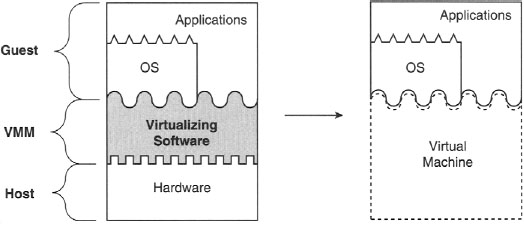
\includegraphics[scale=0.75]{images/fig17.jpg}
	\caption[Sistema  de maquina virtual]{El software de virtualización transforma una plataforma hardware a otro capaz de ejecutar software desarrollado para esa plataforma.}
	\label{fig:1.7}
\end{figure}
La información ha sido extraída del libro \textbf{Virtual Machines: Versatile Platforms for Systems and Processes}\cite{smith2005virtual}.
\subsection{Virtualización con contenedores}
En este tipo de virtualización, también es conocida como virtualización de sistema operativo. La virtualización  se ejecuta como proceso del sistema operativo. Los contenedores, en este caso, serían lo que llamamos en el punto anterior ``invitados''. La diferencia entre este enfoque y las maquinas virtuales completas, es que no se virtualiza el SO de forma completa. En la Figura \ref{fig:hypervisor} podemos ver el enfoque clásico. Donde podemos ver como sobre el SO ``host'' instalamos el hipervisor que es el encargado de ofrecer el hardware a los SO huéspedes. Como vemos se realiza la instalación completa de los sistemas operativos. 
 \begin{figure}[H]
	\centering
	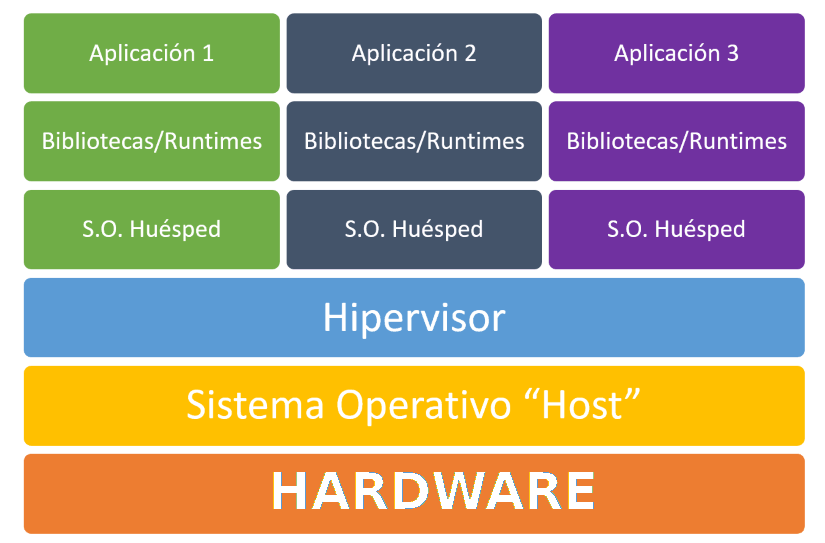
\includegraphics[scale=0.5]{images/estructura_hypervisor.png}
	\caption[Estructura clásica]{Estructura clásica}
	\label{fig:hypervisor}
\end{figure}
La filosofía seguida por los contenedores es diferente.  Se aíslan las aplicaciones en sistemas virtuales, pero no es necesario que alberguen un sistema operativo completo. En el caso de Docker, Docker Engine es el encargado de lanzar y gestionar los contenedores. Este es el que se encarga de gestionar los recursos, optimizando el uso. Además las imágenes de Docker se pueden reutilizar entre diferentes aplicaciones (ver en la Figura \ref{fig:docker}). Por ejemplo podemos tener una imagen de PHP y compartirlo entre dos aplicaciones diferentes, pero aisladas entre ellas.\\\\
Cuando se lanzan varios contenedores a partir de una sola imagen, para nuestra aplicación es como si se estuviera ejecutando en el sistema anfitrión, pero aislado de las demás aplicaciones, cada uno tendrá su propio sistema de archivos. Aunque también es factible que acceda al sistema de ficheros anfitrión, esto es útil para que los datos sean persistentes y aunque se cierre el contenedor, no se pierdan.
\begin{figure}[H]
	\centering
	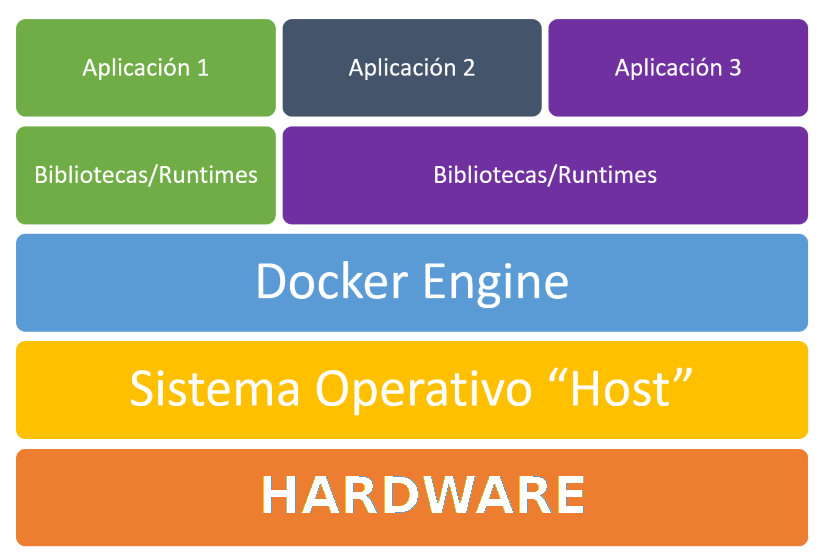
\includegraphics[scale=0.5]{images/estructura_docker_engine.png}
	\caption[Estructura de contenedores]{Estructura clásica}
	\label{fig:docker}
\end{figure}
\section{Análisis}
\subsection{Ventajas}
 En comparación con otras tecnologías de virtualización, Docker destaca en velocidad, portabilidad, escalabilidad, seguridad y optimización de recursos. A continuación, ahondamos en estas ventajas \cite{rad2017introduction}.\\\\
\textbf{Velocidad.} Debido al tamaño reducido de los contenedores, el tiempo requerido para construirlos es breve, lo que permite al usuario desarrollar, probar y desplegar sus proyectos rápidamente. Además, los contenedores permiten ser reutilizados, ahorrando el tiempo de construcción al usuario.\\\\
\textbf{Portabilidad.} Un contenedor Docker se puede ejecutar en cualquier máquina que tenga habilitado Docker. Las aplicaciones incluidas en dichos contenedores no tienen que estar vinculadas al sistema operativo host. Esto permite que se puedan mover fácilmente, como un elemento único sin que el rendimiento disminuya, siempre que el sistema de destino sea compatible con Docker.\\\\
\textbf{Escalabilidad.} Docker tiene la capacidad de desplegarse tanto en servidores físicos como en plataformas en la nube. Los contenedores Docker pueden pasar de un entorno remoto al host local del usuario y desde allí, volver al entorno remoto de nuevo sin mucho esfuerzo. Los ajustes de Docker permiten modificar la escala de los contenedores según la necesidad del usuario.\\\\
\textbf{Seguridad.} Los procesos que se ejecutan en un contenedor Docker están aislados de los procesos que se ejecutan en el sistema operativo o en otros contenedores \cite{merkel2014docker}. Además, el formato de los contenedores Docker está estandarizado para que todos los usuarios pueden trabajar sin tener que preocuparse por las tareas de los demás, es decir, las responsabilidades de cada usuario están bien definidas. Estas responsabilidades hacen que Docker pueda proporcionar un entorno mejorado, confiable y consistente entre los distintos usuarios.\\\\
\textbf{Optimización de recursos.} La principal ventaja respecto a las máquinas virtuales es que Docker no utiliza hipervisor. Esta es la razón por la que se pueden ejecutar muchos más contenedores en un servidor que máquinas virtuales. El rendimiento de los contenedores Docker es mayor debido a un uso eficiente de los recursos: si un contenedor no está ejecutándose, no consume recursos, por lo tanto, el sistema operativo y otros contenedores pueden recurrir a estos recursos libres \cite{merkel2014docker}.\\\\
\subsection{Desventajas}
Sin embargo, Docker también presenta una serie de inconvenientes \cite{merkel2014docker,rad2017introduction}: 
 \begin{itemize}
     \item Actualmente solo es compatible con máquinas locales de 64 bits.
     \item La integración y el rendimiento pueden verse afectados si se utilizan máquinas Windows o Mac.
     \item Hay una posible brecha de seguridad con Docker, ya que actualmente se ejecuta con privilegios de root. Una solución a esto, es utilizar otro tipo de software que no requiera el uso de un demonio, por ejemplo, {\textbf{\emph{Podman}}} (ver sección \ref{ti:podman}).
     \item Aunque el tipo de aislamiento proporcionado es bastante fuerte en general, puede decirse que no es tan fuerte como el que se puede conseguir con la utilización de máquinas virtuales. Si el núcleo falla, también lo harán todos los contenedores.
     \item Docker no tiene la madurez ni la popularidad que tienen las máquinas virtuales en entornos de producción.
 \end{itemize}     

\subsection{Comparativa entre distintas opciones}
Docker es la referencia del segmento de los contenedores, pero esto no significa que sea la única opción viable que tenemos. En este apartado vamos a realizar una comparación entre Docker y otras 3 alternativas. Estas alternativas serán \href{https://coreos.com/rkt/}{RKT}, \href{https://podman.io/whatis.html}{podman} y \href{https://singularity.lbl.gov/}{singularity}.
\subsubsection{RKT}
Se creó con la aspiración de superar a Docker en seguridad y está orientado a aplicaciones en producción debido a estas mejoras de seguridad.

RKT implementa un formato de imágenes abierto y estándar, \emph{App Container}, pero también puede
ejecutar otras imágenes, como las creadas usando el formato propietario de Docker, dando esta opción para los usuarios acostumbrados a este formato.

Otra ventaja de RKT es que está mas orientado al software libre y la comunidad, como por ejemplo ocurre con Linux. Esto hace que los usuarios se impliquen más y ayuden a solucionar problemas y a realizar mejoras. Por el contrario, Docker es un producto privativo, aunque también tiene una gran cantidad de recursos para su comunidad de usuarios.

RKT no tiene un demonio ''init'' centralizado, sino que lanza contenedores directamente desde los comandos del cliente, lo que lo hace compatible con sistemas init como systemd, upstart y otros \cite{rktvsdocker}. Con Docker, los contenedores lanzados no son compatibles con sistemas init.

RKT también es capaz de descargar la imagen del contenedor y la verificación de esta con usuarios sin privilegios, mientras que Docker necesita realizar esto mediante su demonio que necesita permisos de root.

\begin{figure}[H]
	\centering
	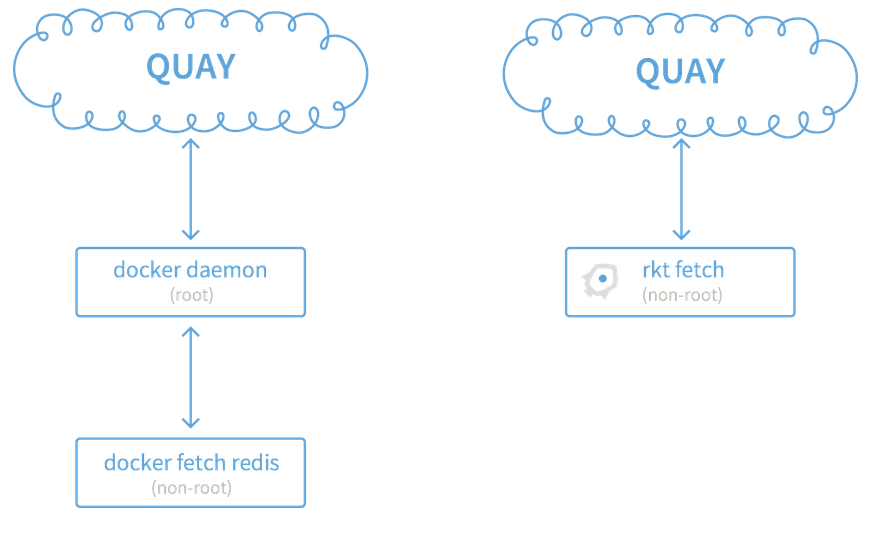
\includegraphics[scale=0.5]{images/crearImagen.png}
	\caption[Descarga de imágenes con Docker y RKT]{Descarga de imágenes con Docker y RKT}
	\label{fig:docker}
\end{figure}

\subsubsection{Podman}\label{ti:podman}
La gran diferencia de Podman con Docker es que este no utiliza un servicio, lo que lo limita al no tener una API SERVICE. Por la falta de esto, tiene limitaciones en lo que puede hacer.
Con Docker, por ejemplo, tenemos gestión de ciclo de vida, que se encarga de reiniciar contenedores en caso de fallos o iniciarlos si se reinicia el equipo, chequeo sobre los contenedores o iniciarlos con un orden especifico. Podman, en cambio, no incluye estos aspectos directamente, de forma que la gestión de los contenedores se tendrá que realizar mediante systemd. 

En cambio, un punto a favor de Podman es que al no tener un servicio, este necesita menos recursos del sistema y puede dedicar mas recursos a los contenedores. Por ejemplo, a la hora de lanzar un contenedor con NGINX, Podman lo hace con un único proceso, mientras Docker necesitar muchos más.

Con esto obtenemos que Podman requiere menos espacio y dependencias que Docker, siendo esta una de sus principales ventajas.

Podman fue diseñado para que cambiar desde Docker a este se realizara de una forma sencilla. Por eso tiene la misma CLI (command-line interface). 

\subsubsection{Singularity}
Como los dos anteriores, también es compatible con las imágenes de Docker. 

Una de las principales diferencias con Docker es la forma de construir los contenedores. No utiliza un servicio como Docker, sino que mediante los permisos de SUID (Set User ID) realiza, como root, las llamadas a sistema necesarias para la creación del contenedor. Una vez creado el contenedor y antes de darle al usuario el control del contenedor, abandona los permisos de root y vuelve a tener los permisos del usuario que convocó la creación del contenedor. 
Singularity también tiene la opción de desplegar un contenedor sin necesitar privilegios de root mediante namespace de usuario, a cambio, estos contenedores tendrán limitadas las funcionalidades del contenedor y la portabilidad del mismo. 

Una de las principales diferencias de Singularity es la forma de interactuar con los contenedores. Mientras que Docker utiliza comandos específicos para trabajar con los contenedores, Singularity utiliza los contenedores como si fueran scripts. Se podría arrancar un contenedor con ./ igual que un script. 

Otro de los aspectos diferentes que tiene Singularity es que tiene acceso a los ficheros del anfitrión sin necesidad de indicarle al contenedor que los monte al crearlo como pasa en Docker. Estos ficheros se podrían pasar, por ejemplo, como parámetro.

Vamos a realizar un ejemplo en el que tenemos un contenedor llamado copiarfichero.sif que necesita dos ficheros para trabajar, estos ficheros se les pasara a la hora de ejecutarlos. El comando seria el siguiente:
\begin{verbatim}

./copiarficheor.sif input.txt output.txt. ­

\end{verbatim}

De esta manera tendríamos una forma mas sencilla de ejecutar los contenedores y de poder utilizar ficheros distintos sin tener que estar indicando en la configuración que estos sean montados al iniciar el contenedor.

\section{Desarrollo: Ejemplos con Docker}
\subsection{Ejemplo 1: LAMP}
En el primer ejemplo vamos a ver la configuración de un contenedor que nos ofrece la pila \href{https://github.com/sprintcube/docker-compose-lamp}{LAMP completa}. Con un solo contenedor tenemos un servidor web y la base de datos. Gracias a ello podremos desplegar rápidamente una aplicación web basada en PHP desde cualquier servicio cloud. Usaremos la herramienta \href{https://docs.docker.com/compose/}{\textbf{docker-compose} }la cual nos permite definir y ejecutar aplicaciones de Docker de varios contenedores. \\\\Para configurar un contenedor con ``docker-compose'' necesitamos definir el fichero ``docker-compose.yml''. En este documento indicaremos cuales otros contenedores vamos a querer y cual es la  configuración de cada uno. Además de este fichero, cada contenedor que indicamos en el docker-compose.yml tiene su propio Dockerfile. Pero para poder usarlos no nos hace falta saber como son, ya que docker-compose no abstrae de toda esa parte. En ejemplos posteriores si indicaremos como se realiza el fichero Dockerfile. \\\\
Fichero ``docker-compose.yml'':
\begin{minted}{yaml}
version: "3"

services:
  webserver:
    build: 
      context: ./bin/webserver
    container_name: '7.4.x-webserver'
    restart: 'always'
    ports:
      - "${HOST_MACHINE_UNSECURE_HOST_PORT}:80"
      - "${HOST_MACHINE_SECURE_HOST_PORT}:443"
    links: 
      - mysql
    volumes: 
       - ${DOCUMENT_ROOT-./www}:/var/www/html
      - ${PHP_INI-./config/php/php.ini}:/usr/local/etc/php/php.ini
      - ${VHOSTS_DIR-./config/vhosts}:/etc/apache2/sites-enabled
      - ${LOG_DIR-./logs/apache2}:/var/log/apache2
  mysql:
    build:
      context: "./bin/${DATABASE}"
    container_name: 'mysql'
    restart: 'always'
    ports:
      - "${HOST_MACHINE_MYSQL_PORT}:3306"
    volumes: 
      - ${MYSQL_DATA_DIR-./data/mysql}:/var/lib/mysql
      - ${MYSQL_LOG_DIR-./logs/mysql}:/var/log/mysql
    environment:
      MYSQL_ROOT_PASSWORD: ${MYSQL_ROOT_PASSWORD}
      MYSQL_DATABASE: ${MYSQL_DATABASE}
      MYSQL_USER: ${MYSQL_USER}
      MYSQL_PASSWORD: ${MYSQL_PASSWORD}
\end{minted}
En el fichero anterior podemos ver como declaramos que haremos uso de dos servicios. Uno que sera el servidor web (webserver) y otro que nos proporcionara la base de datos (mysql). Esos dos contenedores ya nos los dan configurados, solo tenemos que indicarles los puertos de los que hacen uso, nombres de usuario, contraseñas, etc. Como podemos ver, esos datos no están puestos directamente, si no que hacen referencia a ``variables''. Dichas variables las tenemos en el fichero ``.env'', que para evitar sobrecargar, documento solo pondré una parte:
\begin{minted}{yaml}
DOCUMENT_ROOT=../SIBW/Practica4
VHOSTS_DIR=./config/vhosts
APACHE_LOG_DIR=./logs/apache2
PHP_INI=./config/php/php.ini
\end{minted}
Este fichero, simplemente es un diccionario de variables, a la izquierda se encuentra el nombre de la variable y a la derecha su valor.\\
Para ejecutar el contenedor basta con realizar lo que vemos en la Figura \ref{fig:dock}:
\begin{figure}[H]
	\centering
	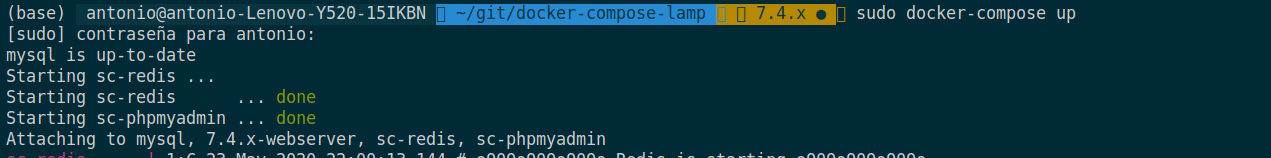
\includegraphics[scale=0.3]{images/docker-compose.png}
	\caption[docker-compose up]{Levantamos el contenedor de la pila LAMP}
	\label{fig:dock}
\end{figure}
Y como podemos ver, podemos acceder desde nuestra maquina anfitrión al servicio que nos ofrece el contenedor en la Figura \ref{fig:serv}.
\begin{figure}[H]
	\centering
	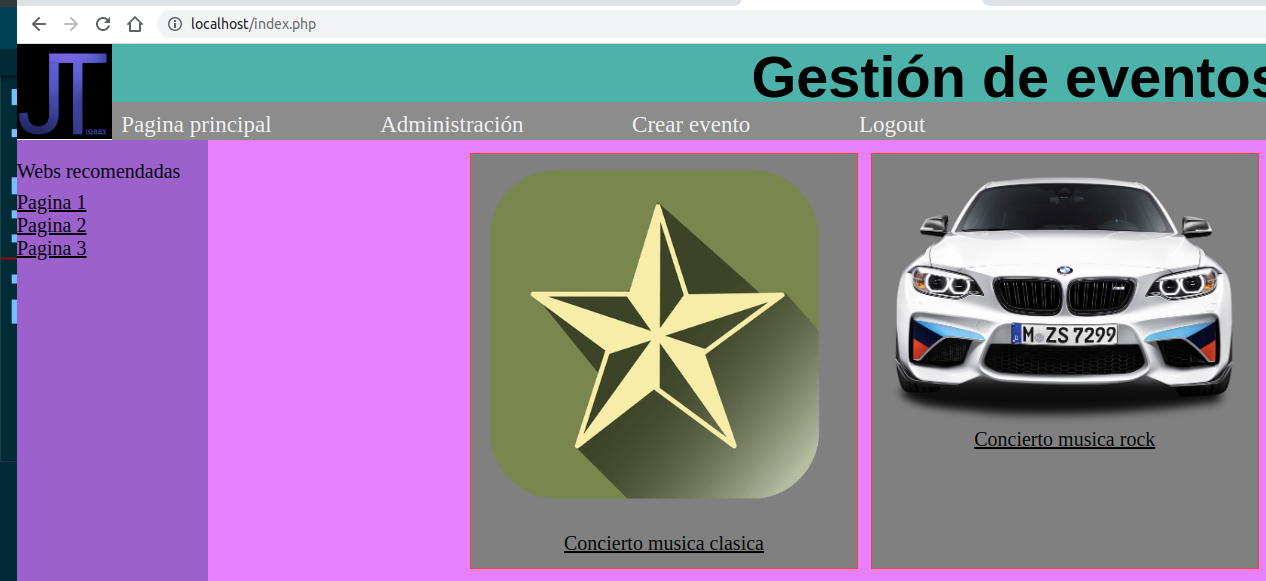
\includegraphics[scale=0.3]{images/a.png}
	\caption[Acceso a la pila LAMP]{Accedemos al contenedor de la pila LAMP}
	\label{fig:dock}
\end{figure}
Y también podríamos tener acceso a la base de datos mediante php-my-admin o desde la consola.
\subsection{Ejemplo 2: Docker + Flask}
En este ejemplo vamos a configurar un contenedor Docker con un servidor web básico utilizando Flask. Se utilizará un equipo Windows como host para ver las diferencias con respecto a Linux. Como este equipo no dispone de Windows Pro, la tecnología \href{https://docs.microsoft.com/es-es/virtualization/hyper-v-on-windows/about/}{Hiper-V} no está disponible, por tanto, deberemos usar un \href{https://docs.docker.com/toolbox/toolbox_install_windows/}{conjunto de herramientas} basadas en VirtualBox para usar Docker.\\\\
En la Figura \ref{fig:E3_1} se puede observar la herramienta Docker Toolbox una vez iniciada.

\begin{figure}[H]
	\centering
	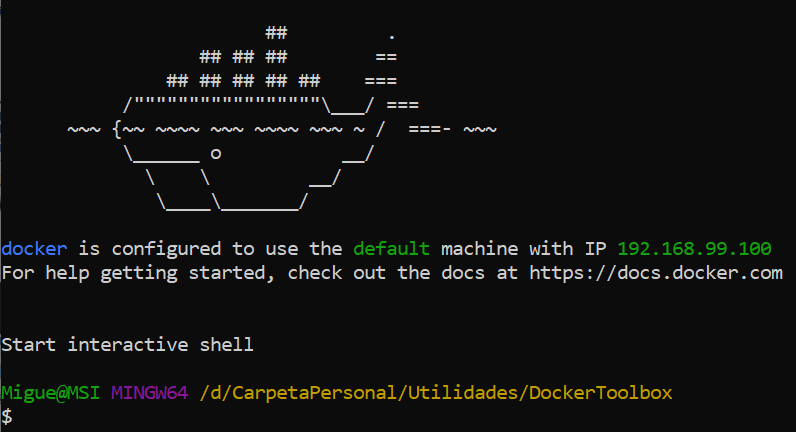
\includegraphics[scale=0.4]{images/E3_1.png}
	\caption[Docker Toolbox para Windows]{Herramienta para manejar Docker en Windows a través de VirtualBox.}
	\label{fig:E3_1}
\end{figure}

Para configurar Docker solo son necesarios dos archivos:
\begin{itemize}
    \item Docker-compose.yml (ver Figura \ref{fig:E3_docker}): En este archivo se configura la versión de Docker que utilizaremos y el servicio que vamos a crear. Para que funcione Flask vamos a crear un servicio web, el cual funcionará a través del puerto 8080. Con la directiva \emph{volumes} podemos montar los directorios y archivos en el contenedor Docker. Con \emph{working-dir} indicamos el directorio de trabajo. 
    \begin{figure}[H]
    	\centering
    	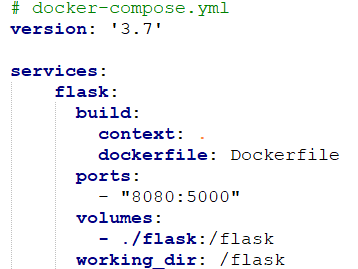
\includegraphics[scale=0.5]{images/E3_docker-compose.PNG}
    	\caption[Docker-compose.yml]{Archivo de configuración del servicio del contenedor Docker.}
    	\label{fig:E3_docker}
    \end{figure}
    \item Dockerfile (ver Figura \ref{fig:E3_dockerfile}): Este archivo lo utilizaremos para instalar y ejecutar todos los archivos que sean necesarios para que funcione nuestro servicio. También lo utilizaremos para activar el modo debug de flask. El archivo \emph{requirements.txt} contiene los paquetes (uno por línea) que se instalarán a través del comando pip, en este ejemplo, solo instalaremos el paquete flask.
    \begin{figure}[H]
    	\centering
    	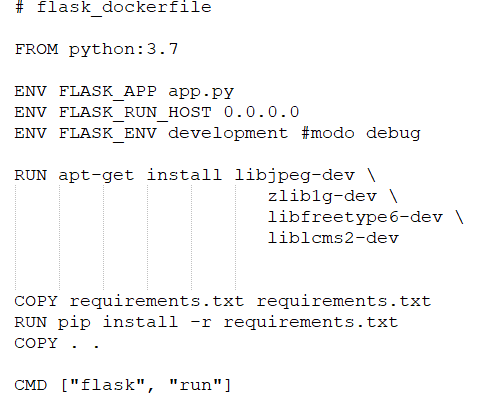
\includegraphics[scale=0.5]{images/E3_dockerfile.PNG}
    	\caption[Dockerfile]{Archivo Dockerfile usado en nuestro ejemplo.}
    	\label{fig:E3_dockerfile}
    \end{figure}
\end{itemize} 
Crearemos un directorio llamado flask, y dentro de el un archivo \emph{app.py}. Este archivo contendrá toda la lógica de nuestra aplicación. En la Figura \ref{fig:E3_app} se muestra este archivo. 
\begin{figure}[H]
	\centering
	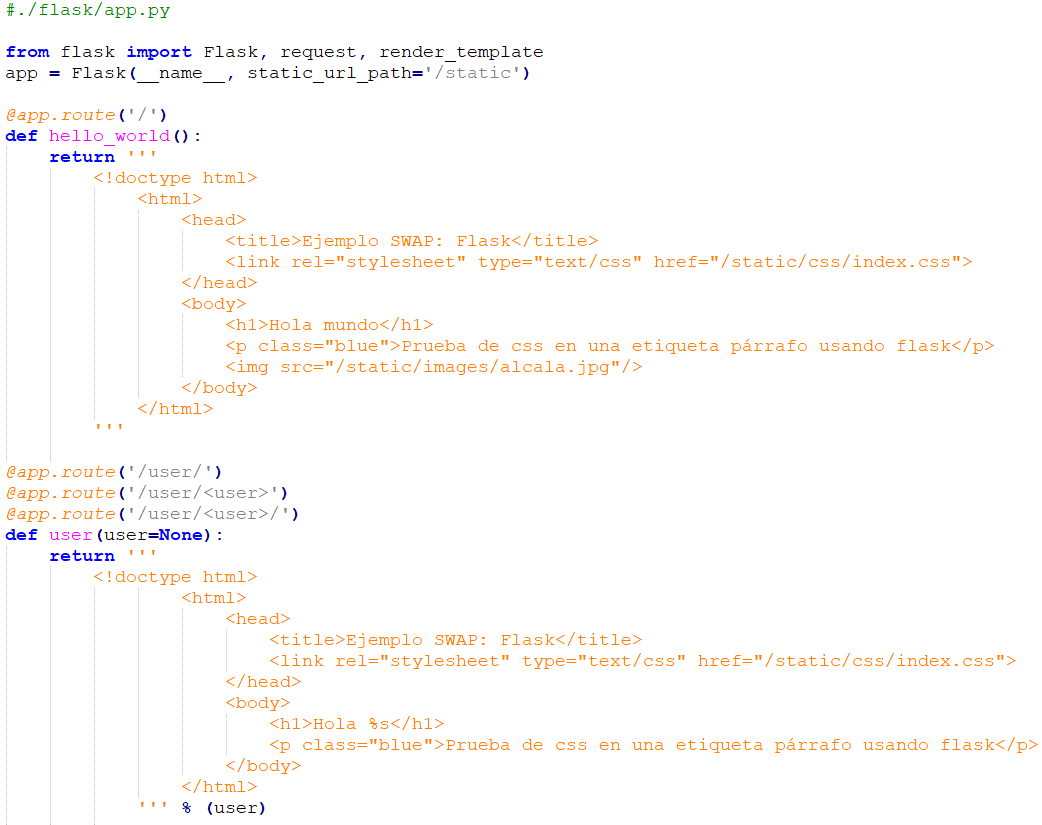
\includegraphics[scale=0.5]{images/E3_app.PNG}
	\caption[app.py]{Archivo con la lógica de nuestra aplicación con Flask.}
	\label{fig:E3_app}
\end{figure}
Desde la consola de Docker, debemos de situarnos en el directorio que hemos creado y utilizar la orden
docker-compose up como en la Figura \ref{fig:E3_docker-up} para iniciar el contenedor.
\begin{figure}[H]
	\centering
	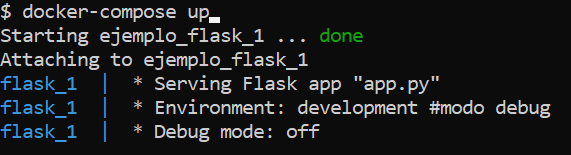
\includegraphics[scale=0.5]{images/E3_docker-up.PNG}
	\caption[docker-compose]{Resultado de iniciar el contenedor creado.}
	\label{fig:E3_docker-up}
\end{figure}
Ya solo nos queda comprobar, mediante el navegador, que nuestra aplicación web está funcionando correctamente. Esta comprobación se puede observar en la Figura \ref{fig:comprobacion}.
\begin{figure}[H]
	\centering
	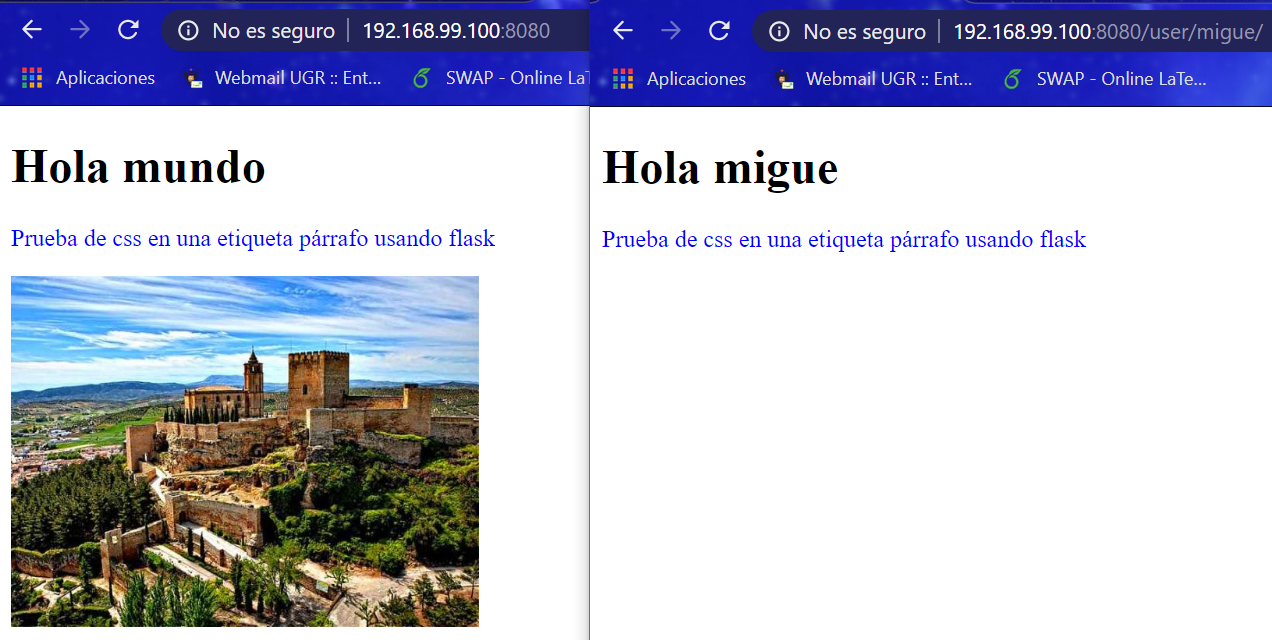
\includegraphics[scale=0.5]{images/E3_comprobacion.PNG}
	\caption[Comprobacion]{Archivo con la lógica de nuestra aplicación con Flask.}
	\label{fig:comprobacion}
\end{figure}
\newpage

\subsection{Ejemplo 3: Singularity}
Vamos a realizar un ejemplo simple con Singularity para demostrar el funcionamiento de las características explicadas anteriormente.
Vamos a crear el fichero que configura nuestro contenedor.
\begin{figure}[H]
	\centering
	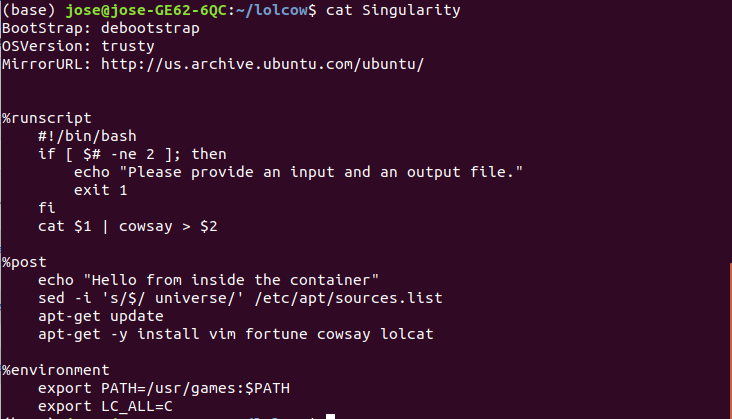
\includegraphics[scale=0.5]{images/configuracionSin.png}
	\caption[Configuración Singularity]{Configuración del contenedor Singularity.}
	\label{fig:configuracionSin}
\end{figure}

La linea BootStrap nos indica el sistema que queremos utilizar, en nuestro caso debootstrap que es una versión de Debian que se ejecuta en una carpeta de otro sistema operativo. En la segunda linea especificamos el sistema operativo sea la versión de Ubuntu Trusty que obtendremos del repositorio que tenemos en la tercera linea. 

En el apartado  \%runscript pondremos el script que queremos que se ejecute cuando lancemos nuestro contenedor. En este caso sera un pequeño script que comprobará si se le pasan dos parámetros, avisando si no se da ese caso, y si se cumple realizará el comando cowsay que nos mostrara el mensaje que pasemos como primer parámetro. Este comando mostrará un burro por consola diciendo el mensaje pasado.

En el apartado \%post se pondrán los comandos que queremos ejecutar después de compilar el sistema operativo. Podrían ser paquetes que queremos que se instalen o cualquier comando que queramos que realice para preparar nuestro contenedor. 

En la sección \%environment configuramos las variables globales que utilizará nuestro sistema. 

Con esto ya tenemos configurado nuestro contenedor. Ahora pasaremos a construirlo con el siguiente comando.
\begin{verbatim}

sudo singularity build --force lolcow.simg Singularity
\end{verbatim}

La opción --force obliga a que nuestro contenedor se reescriba completamente si ya existía. El contenedor se guardará en lolcow.simg y Singularity, en este caso, es el fichero en el que tenemos la configuración. Con esto ya tenemos el contenedor listo para ejecutar. Vamos a mostrar la ejecución de este.

\begin{figure}[H]
	\centering
	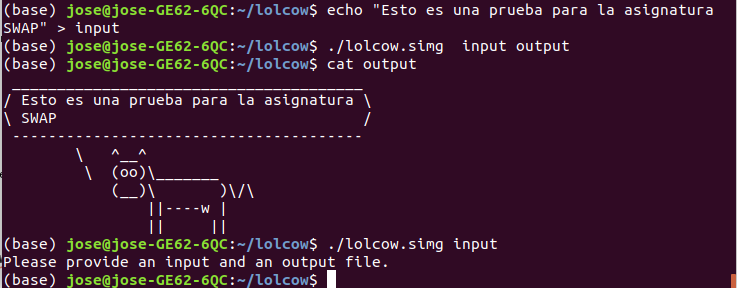
\includegraphics[scale=0.5]{images/ejecucionSin.png}
	\caption[Ejecución Singularity]{Ejecución del contenedor Singularity.}
	\label{fig:ejecucionSin}
\end{figure}

Como vemos se ejecuta el contenedor como si fuera un script con parámetros de entrada. 

\section{Conclusiones}
Podemos resumir que la principal diferencia es que los contenedores se virtualizan a nivel de sistema operativo, mientras que las soluciones basadas en hipervisor se virtualizan a nivel de hardware. Aunque el efecto final que producen ambas es el mismo, las diferencias son importantes y muy significativas.

Aunque sean tan diferentes, estas tecnologías pueden complementarse entre sí, compensando las carencias de una con las virtudes de la otra. Dirk (2014) habla de está posible combinación y utiliza el término \emph{''frenemies''} para referirse a la relación entre los contenedores y las máquinas virtuales \cite{merkel2014docker}. También, en el artículo anterior se comenta que la idea no es encapsular cada aplicación o componente en una máquina virtual, sino implementar fácilmente contenedores Docker dentro de las mismas máquinas virtuales.\\\\
En el mercado Docker ha sido la gran ganadora en el terreno de contenedores. Esto se debe a que tiene detrás un gran equipo dándole soporte y mucha inversión. Es una opción muy fiable que también tiene una gran comunidad que la respalda y crea una gran cantidad de documentación que ayuda a la hora de iniciarte en su utilización. Por el contrario, algunos problemas que ya explicamos en el apartado de comparación dan opciones a la competencia a quitarle parte de la cuota de mercado. Según un estudio de la empresa Sysdig \cite{sysdigUsage}, Docker tenía un total del 83\% del tiempo de uso respecto a la competencia en 2018.

\begin{figure}[H]
	\centering
	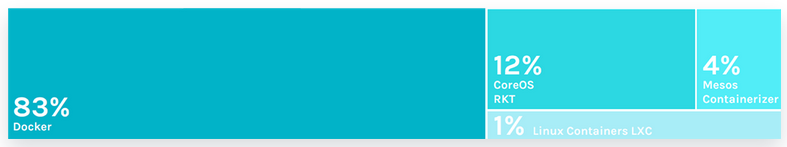
\includegraphics[scale=0.5]{images/usoDocker.png}
	\caption[Estadística de uso de contenedores.]{Estadística de uso de contenedores.}
	\label{fig:usoDocker}
\end{figure}

En este mismo estudio se dice también que en 2017 Docker tenía un 99\%. Con esto vemos como los competidores de Docker están intentando quitarle cuota a este, introduciendo mejoras en las partes donde Docker es más flojo. Esto nos indica, como mencionamos anteriormente, que es un sector en auge, y además, se esta invirtiendo mucho esfuerzo, ya que es muy interesante para las empresas.
\\\\
\clearpage
\newpage
\bibliographystyle{plain}
\bibliography{references}
\end{document}
